\documentclass[12pt, oneside]{article}
\usepackage[letterpaper, margin=1in]{geometry}
\usepackage[english]{babel}
\usepackage[utf8]{inputenc}
\usepackage{amsmath}
\usepackage{amsfonts}
\usepackage{amssymb}
\usepackage{tikz}
\usepackage{tkz-fct}
\usepackage{venndiagram}

\usepackage{fancyhdr}
\pagestyle{fancy}
\fancyhf{}
%\rhead{Name: \hspace{1.5in} }
\lhead{BECA / Dr. Huson / Algebra II \qquad Name:\\* 17 April 2018}

\vspace{1cm}

\renewcommand{\headrulewidth}{0pt}

\title{Worksheet and test template}
\author{Chris Huson}
\date{March 2018}

\begin{document}

\subsubsection*{\\* Problem set: Features of polynomial graphs}
%Write your answers in the space provided. Attach your work on a separate sheet of lined paper, clearly labeling the problems.

\begin{enumerate}

\item The graph of the cubic function $f(x)$ is shown. For each vocabulary word, list the appropriate labels A-F from the graph.
\begin{center}
    \begin{tikzpicture}[scale=2.4/3]
    \draw[thick,<->] (-5.5,0) -- (6.5,0) node[anchor=north west] {\textbf{x}};
    \draw[thick,<->] (0,-3.0) -- (0,5.5) node[anchor=south east] {\textbf{f(x)}};
    %\foreach \x in {-1, 1} \draw (\x cm,5pt) -- (\x cm,-5pt) node[anchor=north] {$\x$};
    \foreach \x in {-5,-4,-3,-2, 2, 3, 4,5,6} \draw (\x cm,5pt) -- (\x cm,-5pt) node[anchor=north] {};
    %\foreach \y in {5} \draw (1pt,\y cm) -- (-1pt,\y cm) node[anchor=east] {50}; %{$\y$};
    \tkzInit[xmin=-5,xmax=5,ymin=-7,ymax=7,ystep=1]   
    \tkzFct[color=black,very thick,<->,domain = -3.4:4.0] {0.2*(x*x-9)*(x-1)};
    \end{tikzpicture}
\end{center}
\begin{enumerate}
    \item The roots\\*
    \item As $x\xrightarrow{}+\infty$, $y\xrightarrow{}+\infty$\\*
    \item $f(0)=y$\\*
    \item The solutions\\*
    \item As $x\xrightarrow{}-\infty$, $y\xrightarrow{}-\infty$\\*
    \item The $y$-intercept\\*
    \item $f(x)=0$\\*
    \item The zeros
\end{enumerate}

\newpage


\item Given a quartic polynomial function $h(x)=(x-4)(x+2)(x+5)(x-1)$. Sketch $y = h(x)$ on the grid below, accurately depicting the $x$- and $y$-intercepts.
\begin{center}
    \begin{tikzpicture}[scale=2.54/4]
    \draw[thick,<->] (-5.5,0) -- (6.5,0) node[anchor=north west] {\textbf{x}};
    \draw[thick,<->] (0,-3.5) -- (0,5.5) node[anchor=south east] {\textbf{y}};
    \foreach \x in {-1, 1} \draw (\x cm,5pt) -- (\x cm,-5pt) node[anchor=north] {$\x$};
    \foreach \x in {-5,-4,-3,-2, 2, 3, 4,5,6} \draw (\x cm,5pt) -- (\x cm,-5pt) node[anchor=north] {};
    %\foreach \y in {5} \draw (1pt,\y cm) -- (-1pt,\y cm) node[anchor=east] {50}; %{$\y$};
    %\tkzInit[xmin=-5,xmax=5,ymin=-7,ymax=7,ystep=1]   
    %\tkzFct[color=black,very thick,<->,domain = -2.5:5] {0.2*(x*x-4)*(x-4)};
    \end{tikzpicture}
\end{center}

\item Given $3x(2x^2+3x+7)=6x^3+hx^2+kx$. Find $h$ and $k$.\\[60pt]

\item Given the function $f(x)=(x+3)(x^2-3x+2)$
\begin{enumerate}
    \item Express $f$ in fully factored form.\\[50pt]
    \item What are the zeros of the function?
\end{enumerate}

\newpage
\item The graph of the cubic function $f(x)$ is shown. The leading coefficient of $f$ is one.
\begin{enumerate}
    \item What are the roots of $f(x)$?\\*[5pt]
    \item Express $f(x)$ as a polynomial in standard form.\\*[5pt]
    \item Find the $y$-intercept of $f$
\end{enumerate}
\begin{center}
    \begin{tikzpicture}[scale=2.4/4]
    \draw[thick,<->] (-5.5,0) -- (6.5,0) node[anchor=north west] {\textbf{x}};
    \draw[thick,<->] (0,-2.0) -- (0,5.5) node[anchor=south east] {\textbf{f(x)}};
    \foreach \x in {-1, 1} \draw (\x cm,5pt) -- (\x cm,-5pt) node[anchor=north] {$\x$};
    \foreach \x in {-5,-4,-3,-2, 2, 3, 4,5,6} \draw (\x cm,5pt) -- (\x cm,-5pt) node[anchor=north] {};
    %\foreach \y in {5} \draw (1pt,\y cm) -- (-1pt,\y cm) node[anchor=east] {50}; %{$\y$};
    \tkzInit[xmin=-5,xmax=6,ymin=-7,ymax=7,ystep=1]   
    \tkzFct[color=black,very thick,<->,domain = -2.2:5.5] {0.2*(x*x-4)*(x-5)};
    \end{tikzpicture}
\end{center}

\item What is the quotient when $x^2-3x-40$ is divided by $x + 5$?\\*[25pt]

\item What are the quotient and remainder when $x^3+3x^2-x+2$ is divided by $x - 1$?\\*[25pt]

\item Given the function $f(x)=(x-1)(x+3)$. State the $x$-intercepts of the graph of $f$. Find the $y$-intercept of the graph of $f$.\\*[25pt]


\item If $(x-3)$ is a factor of $f(x)=(x-3)(ax^2+bx+c)$, then what is the value of $f(3)$?\\*[15pt]
\newpage

\item Graph $\displaystyle g(x)= 125(1.08)^ {\frac{10x}{4}} + 75$ on the set of axes below.
\begin{center}
    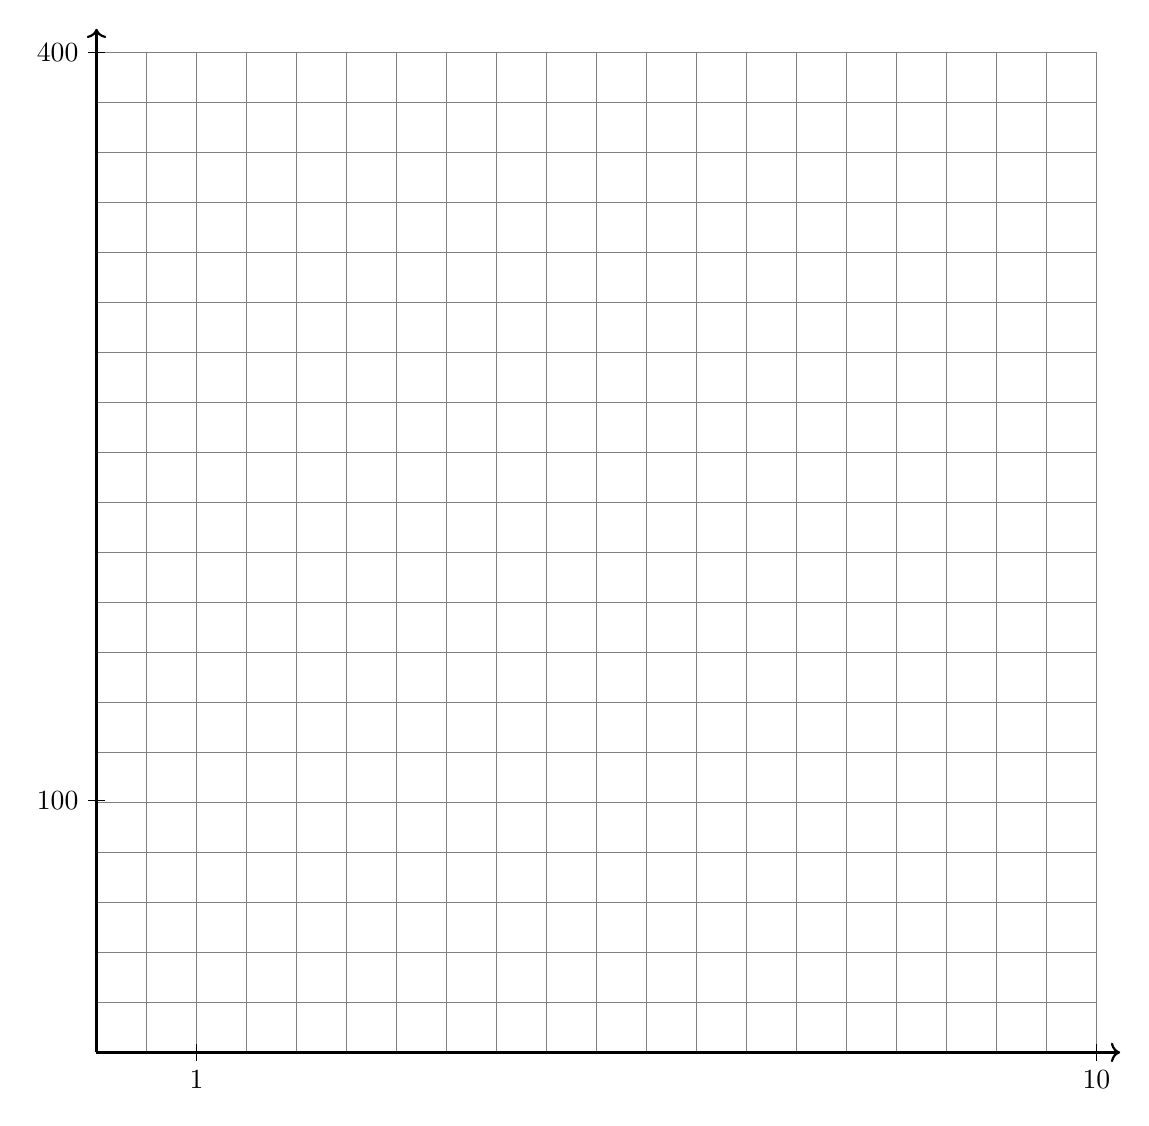
\begin{tikzpicture}
    \draw[step=0.25in,gray,very thin] (0,0) grid (12.7,12.7);
    \draw[thick,->] (0,0) -- (13,0); node[anchor=north west] {x};
    \draw[thick,->] (0,0) -- (0,13); node[anchor=south east] {y};
    \foreach \x in {1.27} \draw (\x cm,3pt) -- (\x cm,-3pt) node[anchor=north] {$1$};
    \foreach \x in {12.7} \draw (\x cm,3pt) -- (\x cm,-3pt) node[anchor=north] {10};
    \foreach \y in {3.2} \draw (3pt,\y cm) -- (-3pt,\y cm) node[anchor=east] {100};
    \foreach \y in {12.7} \draw (3pt,\y cm) -- (-3pt,\y cm) node[anchor=east] {400};
    \end{tikzpicture}
\end{center} %Alg2 Regents Jun2017
Is the function an example of exponential growth or exponential decay? Justify your answer algebraically.

\item Explain why the expression $\displaystyle 16^{\frac{3}{4}}$ is equivalent  according to the rules of fractional exponents. 


\newpage
\item What is the quotient when $x^2-3x-40$ is divided by $x + 5$?\\*[25pt]

\item What are the quotient and remainder when $x^3+3x^2-x+2$ is divided by $x - 1$?\\*[25pt]

\item Given the function $f(x)=(x-1)(x+3)$. State the $x$-intercepts of the graph of $f$. Find the $y$-intercept of the graph of $f$.\\*[25pt]


\item If $(x-3)$ is a factor of $f(x)=(x-3)(ax^2+bx+c)$, then what is the value of $f(3)$?\\*[15pt]

\item When $g(x)$ is divided by $x+4$, the remainder is 0. Given $g(x)=x^4+3x^3- 6x^2- 6x-8$. Write down the value of $g(-4)$.\\*[20pt]

\item Using the quadratic formula or otherwise, find the solution set for $2x^2-3x-5=0$.\\*[20pt]

\item Simplify the expression $\sqrt{a} \cdot \sqrt{a^5}$ \\*[10pt]

\item Simplify the expression $\displaystyle \left( \frac{x^{-2}}{x^2} \right)^{\frac{1}{2}}$ to one with positive integer exponents and radicals.\\*[40pt]

\item Simplify the expression $(-3+2i)(4+3i)$.

\item Simplify the expression $2xi(4+3i)$.\\*[20pt]

\item Let $A$ and $B$ be independent events, where $\mathrm P(A)=0.5$ and $\mathrm P(B)=0.6$.
\begin{enumerate}
    \item Find $\mathrm P(A \cap B)$\\*[20pt]
    \item Find $\mathrm P(A \cup B)$\\*[30pt]
    \item Shade the area representing $A \cap B'$ in Venn diagram below.\\*
        \begin{venndiagram2sets}[tikzoptions={scale=1.2}]
        \end{venndiagram2sets}
\end{enumerate}

\item Use long division to determine the quotient and remainder of $f(x)=(x^3+4x^2-8x-6)$ divided by $g(x)=(x+2)$. Express your answer as $\displaystyle q(x)+\frac{r(x)}{g(x)}$\\*[20pt]



\end{enumerate}
\end{document}